

%\begin{document}

\subsection{A organização GS1}	
	O uso da tecnologia RFID está em crescente expansão, principalmente em aplicações de Supply Chain Management (SCM), no qual saber a localização de cada item da cadeia produtiva é crucial para garantir maior eficácia e eficiência de todo um sistema. Devido essa crescente adoção do RFID, fica constatado que o surgimento de um conjunto de normas que visem à padronização das tecnlogias usadas seria algo natural de se acontecer. Imagine a situação em que uma grande empresa do setor de varejo se funda com outra do mesmo setor, sendo que ambas usam RFID para a localização dos produtos. Se, por exemplo, o formato das TAGs utlizadas pelas empresas forem diferentes, já teremos uma enorme dificuldade de integrar as informações oriundas de cada sistema. Para contornar esse tipo de problema, existe o \textbf{GS1}.
	
	O GS1 é uma organização internacional neutra e sem fins lucrativos, que desenvolve e mantém padrões para cadeias de demanda e suprimentos de diversos setores produtivos. Ele atua principalmente nas áreas de bens do consumo e varejo, saúde e transporte e logística. Algumas empresas que trabalham com o GS1 são: Carrefour, amazon, Google e Coca Cola. 	
	O GS1 foi fundado na década de 70 pelos líderes da indústria dos EUA, tendo com sua primeira atividade a criação do padrão de código de barras conhecido como \textbf{GS1 barcode}, o qual é largamente utilizado até hoje. Com os avanços da tecnologia e seu crescente uso, em 2004 o GS1 criou o primeiro padrão para o RFID.

	O padrão GS1 é divido em três grupos: Identificar, Capturar e Compartilhar. 
	\begin{figure}[h!]
		\centering
		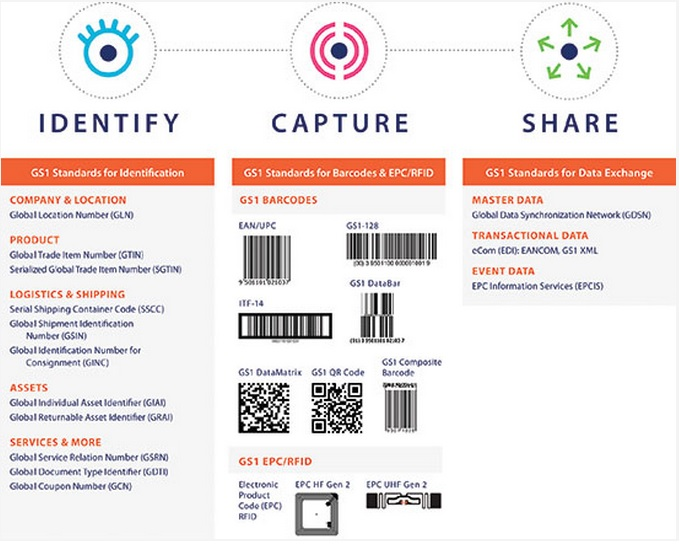
\includegraphics[width=0.7\linewidth]{gs1arch}
		\caption{Grupos do padrão GS1}
		\label{fig:gs1arch}
	\end{figure}

	\paragraph{Identificar} Define códigos de identificação únicos que podem ser usados por um sistema de informação para se referir sem ambiguidade a qualquer tipo de produto.
	\paragraph{Capturar} Inclui definições de códigos de barra e RFID, além de especificar padrões para interfaces entre os elementos de software e hardware que se conectam às aplicações empresariais.
	\paragraph{Compartilhar} Define padrões para o formato dos dados trocados entre as aplicações e os clientes.     

	A norma voltada para aplicações com RFID se enquadra no grupo "Capturar", e suas definições estão presentes no \textbf{EPCGlobal}.


\subsection{O padrão EPCGlobal}
	O padrão EPCglobal é uma iniciatia do GS1 para desevolver padrões voltados à indústria para o EPC, com o objetivo de dar suporte ao uso de RFID. Ele é divido em duas partes: \textbf{EPC/RFID Tags} e \textbf{EPCIS}. 
	
	O EPC (Electronic Product Code) é responsável por interligar o mundo do RFID com os códigos de barra do padrão GS1. Isso funciona da seguinte forma:
		\begin{figure}[h!]
			\centering
			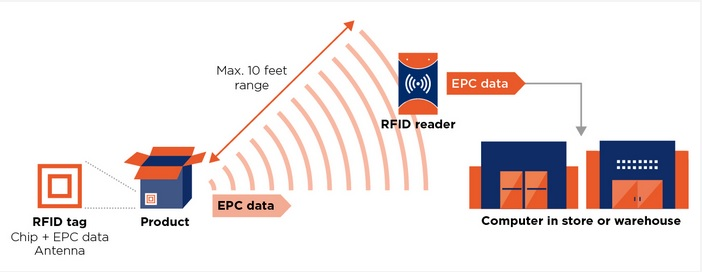
\includegraphics[width=0.5\linewidth]{epcrfid}
			\caption{Funcionamento do EPC}
			\label{fig:epcrfid}
		\end{figure}
	
	Cada produto contém um chip de memória contendo um EPC, o qual consiste de um número de série único. Em cada chip também há uma antena de rádio que transmite o EPC para um leitor RFID quando requisitado. Os dados capturados pelo leitor são então disponibilizados para os outros sistemas.
	
	
	\begin{figure}[h!]
		\centering
		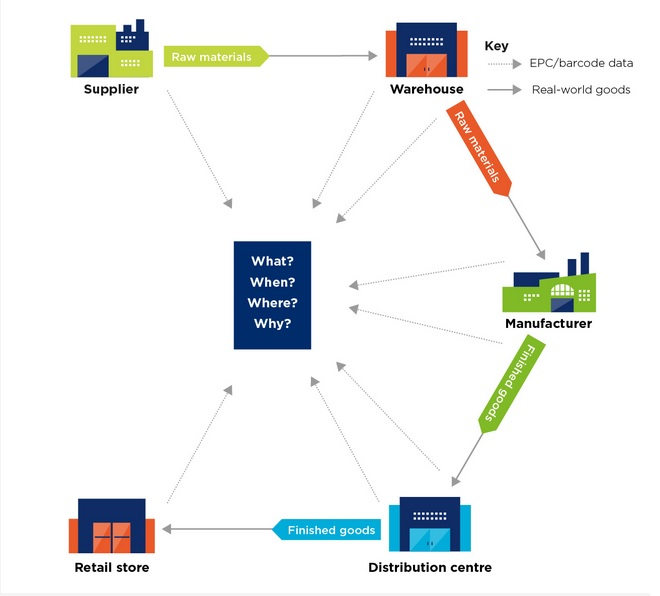
\includegraphics[width=0.5\linewidth]{epcis}
		\caption{Funcionamento do EPCIS}
		\label{fig:epcis}
	\end{figure}
	
	% Falar sobre o EPCIS
	O EPCIS (Electronic Product Code Information Services) é o padrão que habilita as empresas parceiras a compartilhar informações sobre o movimento físico e status dos produtos enquanto eles trafegam pela linha de suprimentos. Uma vez que os dados EPC são coletados, como na figura \ref{fig:epcrfid}, eles são disponibilizados à camada de negócios e todos que possuem acesso a este podem saber o histórico de movimento dos produtos. 
	
	\subsubsection{Arquitetura}

	O EPCGlobal define somente as interfaces, deixando as questões relativas à implementação sobre responsabilidade do usuário. Isso garante uma maior flexiblidade e alimenta o mercado de soluções em sistemas de informação para alcançar essa integração dos dados da cadeia produtiva. A figura \ref{fig:epcarc} apresenta um diagrama contendo a arquitetura básica de um sistema operando com a norma EPCGlobal.

	\begin{figure}[h!]
		\centering
		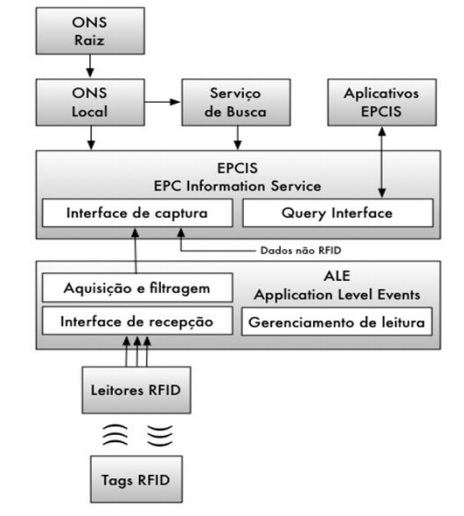
\includegraphics[width=0.5\linewidth]{epcarc}
		\caption{Arquitetura do EPCGlobal. Retirada de \cite{epcSobCug} }
		\label{fig:epcarc}
	\end{figure}
	
	A primeira camada contém os elementos necessários que permitem a identificação única de cada elemento da cadeia produtiva. Ela é composta pelo EPC, Tags e leitores RFID. Nela estão definidos os aspectos de mais baixo nível, como a frequência de operação dos leitores e Tags RFID. Além disso, deve-se especificar a codificação utilizada pelos códigos EPC, pois existem várias codificações, as quais variam de acordo com a aplicação.
	
	Entre os leitores RFID e as aplicações de captura de dados está a interface ALE (Application Level Events). A ALE é uma camada de \textit{Middleware}, responsável por oferecer uma interface de alto-nível às aplicações capaz de agregar dados de diversos leitores, filtrá-los para remover redundâncias, como leituras múltiplas e não-desejadas, e disponibilizá-los de maneira que as aplicações possam trabalhar mais facilmente com esses dados. Resumindo, a ALE é uma interface de pré-processamento de dados, que elimina a necessidade das aplicações de captura de dados lidarem com os aspectos de baixo nível da leitura de dados.
	
	Acima da ALE, temos o EPCIS. Esta é uma interface entre a captura de dados e as aplicações de nível empresarial. A troca de dados provenientes da ALE é feita através de mensagens XML padronizadas, tornando possível o uso do protocolo \textit{SOAP}. O compartilhamento destes dados para o público consumidor e/ou parceiros de negócios é definido pelas empresas, as quais decidem o grau com que elas irão disponiblizar essa informações. Este serviço é garantida pela \textit{Query Interface}, a qual integra os sistemas através de \textit{web services}, utilizando para isto os conceitos do \textit{SOA}. 
	
	Nas camadas mais superiores temos o Object Name Services (ONS), o qual é responsável por descobrir informações sobre um objeto com base no EPC. Para um dado EPC, a URL ou IP associado é pesquisado no banco de dados e os dados referentes àquele objeto podem ser econtrados e devolvidos à quem o requisitou. Ele funciona de maneira análoga a um servidor DNS, o qual traduz domínios em endereços IP.
	
	\subsubsection{Exemplo de aplicação prática}
	O padrão EPCGlobal vem continuamente sendo adotado por diversas empresas na tentativa de aprimorar o processo de visibilidade da cadeia produtiva através do uso de RFID. Como citado anteriormente, grandes empresas estão aderidndo a este padrão e portanto conseguindo uma integração ainda melhor entre os diversos sistemas de informação. Isso pode ser comprovado através do seguinte caso de estudo, que mostra os ganhos obtidos com o advento desta padronização. 
	
	Uma aplicação muito interessante foi desenvolvida na Austrália, chamada \textit{The National Demonstrator Project}. Para isso, foi criado um consórcio de empresas chamado \textbf{CSIRO}, o qual era composto por empresas de renome mundial, como a Gillette, Sun Microsystems, VerySign e a P\&G, além de outras empresas locais de médio e pequeno porte. Seus objetivos principais foram demonstrar o princípio da rede EPC através de sua implementação em toda uma cadeia produtiva, evidenciando os benefícios que esta integração gera para todos os participantes do sistema. 
	
	O processo consistia em monitorar a movimentação de peletes (figura \ref{fig:palete}) entre fornecedores e consumidores, ou de retorno dos paletes de consumidores a fornecedores. Para isto, foram instalados leitores EPC/RFID em todos os galpões, de forma a localizar todos os paletes durante o processo.
	
	\begin{figure}[h!]
		\centering
		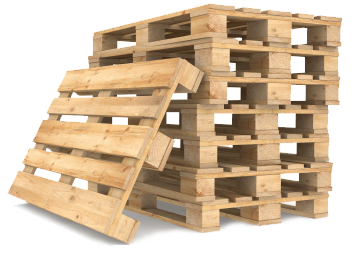
\includegraphics[width=0.2\linewidth]{pallet}
		\caption{Paletes}
		\label{fig:palete}
	\end{figure}

	Ao todo, foram usados 6 galpões, listados na figura \ref{fig:sites}, entre os quais os paletes eram trocados.
	
	\begin{figure}[h!]
		\centering
		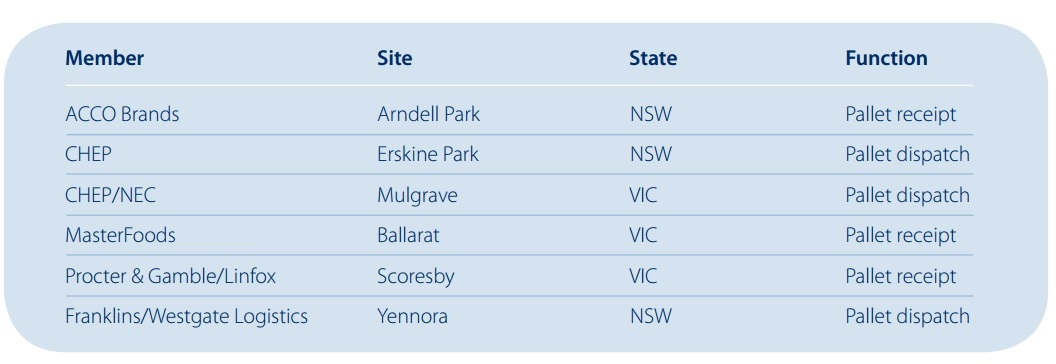
\includegraphics[width=0.6\linewidth]{sites}
		\caption{Galpões utlizados}
		\label{fig:sites}
	\end{figure}
		
	 
	O processo era composto de 9 etapas:
	\begin{enumerate}
		\item O processo inicia quando um cliente gera uma ordem no ERP da CHEP;  
		\item CHEP ou cliente pegam os paletes;
		\item As Tags dos paletes passam pelos leitores RFID e sua localização é gravada no sistema;
		\item Os paletes são despachados para os clientes;
		\item Paletas são recebidas no local desejado
		\item Novamente, as Tags dos paletes passam pelos leitores RFID e têm sua localização salva no sistema;
		\item As Tags são contadas e comparadas com a ordem gerada, salvando os dados no sistema;
		\item Se a quantidade fosse correta, a ordem era aceita. Caso houvesse algum erro, o fornecedor era imediatamente notificado.
	\end{enumerate}	
	
	Isso foi reazliado de maneira completamente automatizada, sem a necessidade de papel e livre de erro humano, melhorando de forma significativa a qualidade do processo. A qualquer momento, é possível acessar o sistema e saber em detalhes a trajetória de cada palete desde o forncedor até o cliente. Mais detalhes da implementação podem ser vistas em \cite{case_epc_demo_ext}.
	
	
	A figura \ref{fig:ausarq} apresenta a arquitetura utilizada para a implementação do projeto. Observe que todas as interfaces definidas anteriormente estão presentes, conforme requerido pela norma. Além disso, os detalhes de implementação não são especificados, o que permitiu ao consórcio, em parceria com a GS1 Austrália uma maior flexibilidade nas decisões relacionadas a esta tarefa.
	
	\begin{figure}[h!]
		\centering
		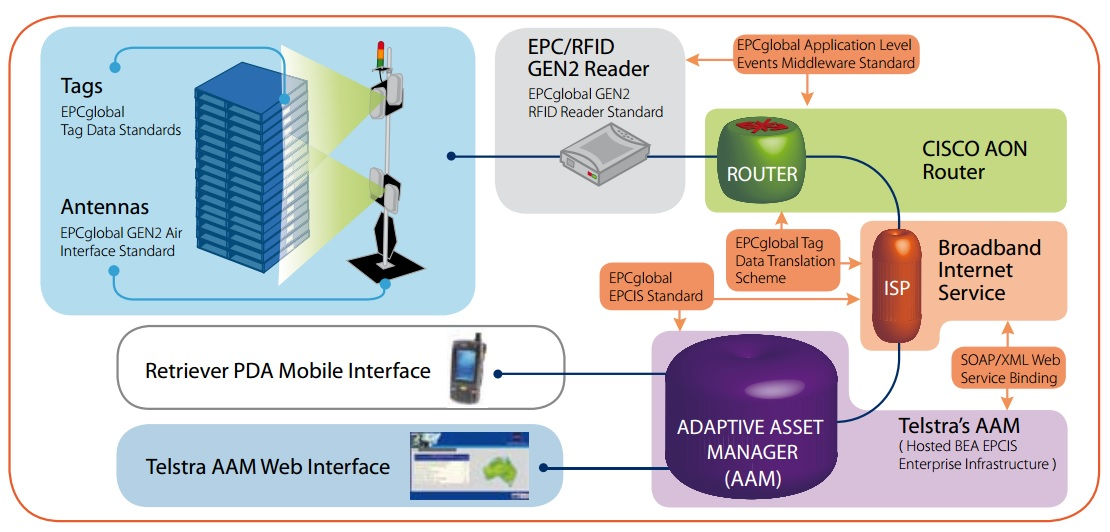
\includegraphics[width=0.7\linewidth]{ausarq}
		\caption{Aquitetura do projeto}
		\label{fig:ausarq}
	\end{figure}
	
	Para avaliar a performance do sistema, foram usados os seguintes critérios:
	\begin{itemize}
		\item Precisão das resultados da leitura de EPC/RFID;
		\item Qualidade: medida através de pesquisa com os membros do consórcio, coletando informações sobre tempo gasto para corrigir erros e para garantir precisão do processo;
		\item Produtividade: comparação entre o processo tradicional e a nova abordagem apresentada neste projeto;
		\item Eficiência: medida pela redução do esforço de trabalho gasto nos processos que anteriormente eram manuais.
	\end{itemize}
	
	Através da medida destes critérios, obteve-se os seguintes resultados:
	\begin{itemize}
		\item Taxas de 100\% de precisão não foram inicialmente obtidas. Fatores como a qualidade e posição das Tags e leitores RFID influenciaram nesse resultado. Após ajustes finos, melhorou-se esta taxa, atingindo valores próximos de 100\%;
		\item Através da pesquisa constatou-se que o tempo gasto encontrando e solucionando erros foi reduzido. Além disso, notou-se um aumento na eficiência no serviço ao consumidor, eliminaçao de operações não produtivas e melhoras no planejamento de manutenção preventiva.
		\item Redução do tempo de processamento entre 5 a 10 minutos, com ganhos de eficiência na faixa de 14.3\% a 22.2\% 
		\item Simplifição significativa, eliminando várias etapas manuais do processo.
		
	Dessa forma, podemos concluir que a adoção da rede EPCGlobal na automatização deste processo atingiu os objetivos estabelecidos, demonstrando que aplicações usando esta norma têm muito a acrescentar às empresas que desejam adotar esta modalidade de integração de dados.
		
	\end{itemize} 
	
	
	\subsection{Considerações Finais}
	Neste seção foi dada uma breve descrição sobre a norma EPCGlobal, mantida e criada pelo consórcio GS1, com enfoque nos aspectos que mais se relacionavam com o conteúdo da disciplina, pois a norma é bem extensa. Aspectos além do escopo deste trabalho ou que não foram explicados de maneira completa podem ser estudados e melhor entendidos  em \cite{gs1} e \cite{gs1arc}. Através do estudo de caso apresentado, podemos conlcuir que esta norma, se aplicada corretamente, funciona na prática e pode entregar bons resultados. Sua utilização pela indústria só tem a agregar valor às aplicações voltadas para o gerenciamento de cadeias de suprimento.
	
%\newpage

%\bibliographystyle{plain}
%\nocite{*}
%\bibliography{biblio_doc}

		
%\end{document}